
%-------------------------------------------------------------
%				INTRODUZIONE
%-------------------------------------------------------------

\mcchap{Introduzione}{cap:intro}

Il progetto in discussione è stato sviluppato durante il periodo di  alto apprendistato presso 7Pixel,
dove sono stato assegnato al team Iguana, team che si occupa
della gestione, principalmente front-end, dei siti del \emph{Kirivo Network}

\section{Il Kirivo Network}
Il Kirivo Network (KN) è attualmente composto da due siti  \url{www.kirivo.it} 
e \url{www.origini.it}:

\url{www.kirivo.it} è un negozio online che vende prodotti di tutte le categorie.
Il marketplace dispone di un offerta di oltre 800.000 articoli in tutte le categorie tra cui
elettrodomestici, prodotti per la casa, smartphone e TV, giocattoli, moda e altri.

\url{www.kirivo.it} è il marketplace ufficiale di \url{www.trovaprezzi.it}, il principale motore
di ricerca italiano per la comparazione di prezzi.

\url{www.origini.it} è una divisione verticale di Kirivo. Il sito è specializzato nella vendita
di vini e offre un ampia offerta di prodotti divisi per cantine e regioni. Il sito
è online da Novembre 2016.

I siti del Kirivo Network fanno utilizzo di servizi di Back-End comuni che permettono 
di effettuare acquisti nei due siti utilizzando un unico account ed un unico carrello.

Con buone probabilità verranno aggiunti in futuro nuovi siti verticali per alcune categorie
di Kirivo.

\section{Architettura del Kirivo Network}
Per l'erogazione dei siti del Kirivo network vengono usati diversi server:
\begin{itemize}
\item {\bf Hybris}: una piattaforma Enterprise di e-commerce scritta in Java che offre una soluzione all-in-one per i siti 
di e-commerce comprendendo servizi quali la gestione del catalogo dei prodotti, degli utenti e la 
gestione sicura dei pagamenti. La scelta di utilizzare una piattaforma di e-commerce a pagamento è stata fatta
principalmente per velocizzare i tempi di sviluppo in fase iniziale.

Hybris utilizza una database relazionale Postgres e il suo catalogo viene indicizzato dal motore di ricerca SolR.

\item {\bf SolR}: un motore di ricerca scritto in Java che permette di indicizzare i prodotti presenti a catalogo per una accesso
più rapido.

Permette inoltre di filtrare in modo efficente i prodotti presenti a catalogo ottimizzando
le ricerche per categorie o caratteristiche del prodotto.

\item {\bf Kiruby}: un web-server Ruby che eroga le pagine web dei siti, si interfaccia con Hybris e Solr utilizzando i loro
servizi di backend. 
\item {\bf Wordpress}: usato per la creazione di pagine di contenuto che vengono incluse da Kiruby.

Il server di Wordpress si trova nella LAN aziendale ed è accessibile solamente dall server Kiruby, la sua
presenza è nascosta agli utenti finali.
\item {\bf Redis}: un database noSql che, salvando tutto il suo contenuto in RAM, garantisce alte prestazioni.

Viene usato da Kiruby come cache di contenuti, specialmente per le richieste di Kiruby a Wordpress.

\item {\bf Nginx}: un Reverse proxy usato per redirigere le chiamate fatte ai domini \url{www.kirivo.it} 
e \url{www.origini.it} ai server opportuni.
\end{itemize}

\begin{figure}
  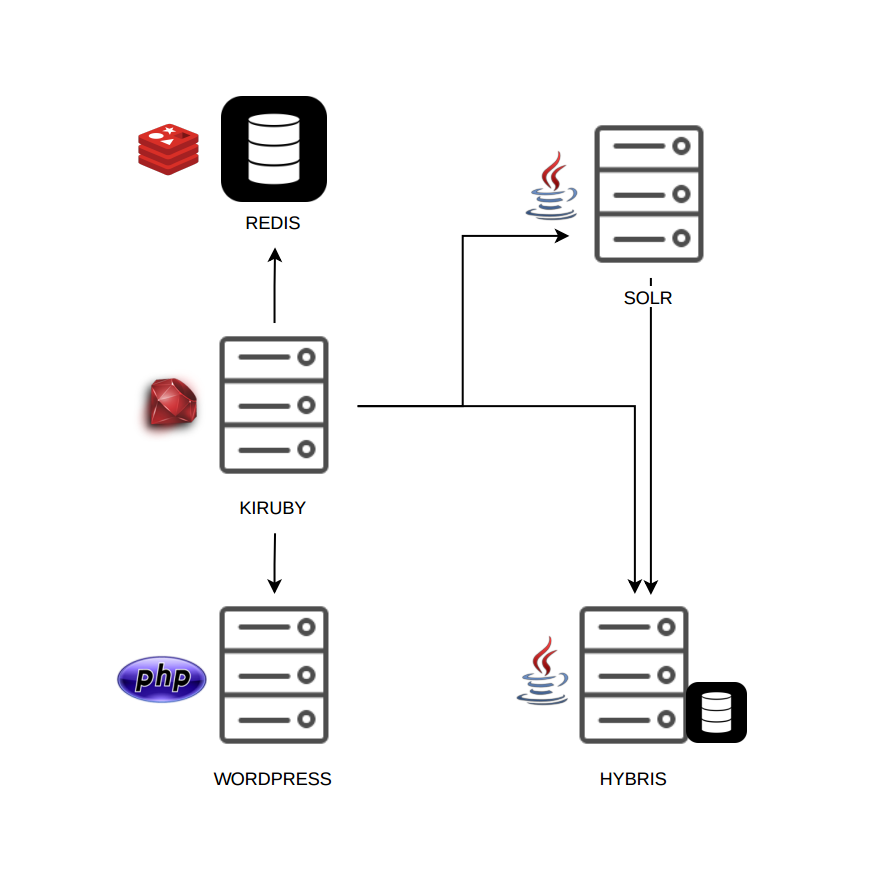
\includegraphics[width=\textwidth]{figure/arch.png}
  \caption{Schema dell'architettura del Kirivo Network.}
  \label{fig:kn}
\end{figure}


\newpage

\section{I team del Kirivo Network}
Lo sviluppo è l manutenzione dei siti del Kirivo Network viene effettuato da più team e questi sono:
\begin{itemize}
\item {\bf Team Iguana}: si occupa dello sviluppo di Kiruby.
\item {\bf Team Nimbus}: si occupa dello svliuppo di Hybris SolR e Kitty.
\item {\bf Content Managers}: si occupano della comunicazione con i venditori, della gestione dei prodotti a catologo
 e della creazione di pagine di speciali, lavorano interfacciandosi con Hybris e Wordpress.
\item {\bf Grafica}: lavora o direttamente su Kiruby o da al team Iguana grafiche HTML che vengono poi rese dinamiche 
ed integrate con i vari servizi.
\end{itemize}

\section{Gestione delle homepage} 	

Le homepage di Origini e Kirivo sono le pagine che, nei rispettivi siti, possono cambiare contenuto più 
frequentemente. Inoltre scegliere quali prodotti, quali offerte e quali contenuti 
vanno inseriti in homepage non è compito dei programmatori ma dei \emph{content managers},
quindi si rivela importante dare la possibilità ai \emph{content} di fare modifiche, come cambiare un prodotto da
mettere tra quelli in evidenza in homepage o il testo di un pannello con la cantina del mese, senza dover passare 
dai programmatori per fare modifiche.

Per dare più libertà ai \emph{content}, il contenuto della homepage, ovvero tutto quello che non è
header e footer, non si trova nel server Kiruby ma in pagine Wordpress che i content possono direttamente 
modificare accedendo alla sezione \emph{admin} di Wordpress.

\begin{figure}
  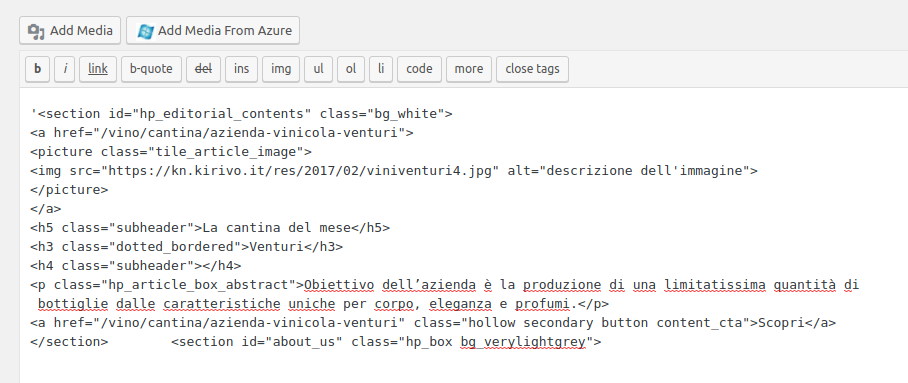
\includegraphics[width=\textwidth]{figure/whtml.png}
  \caption{L'interfaccia visualizzata dai content managers per modificare la pagina.}
  \label{fig:whtml}
\end{figure}

\begin{figure}
  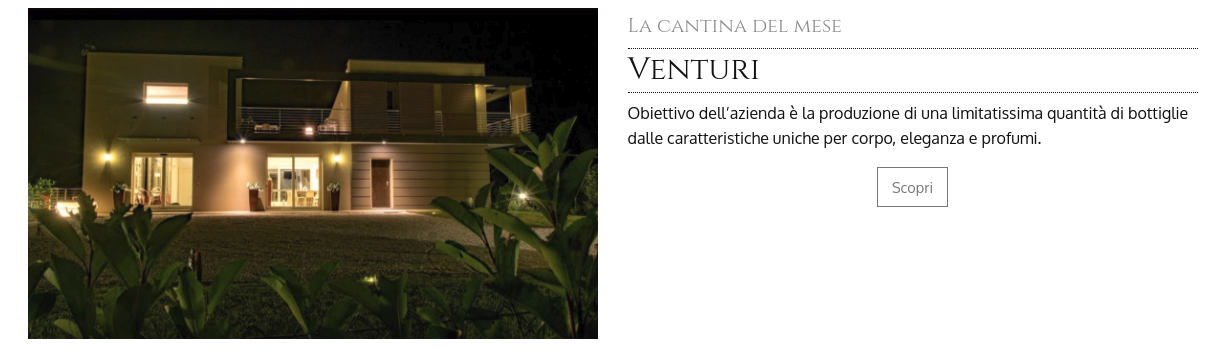
\includegraphics[width=\textwidth]{figure/wrender.png}
  \caption{Risultato renderizzato della componente compilata in figura \ref{fig:whtml}.}
  \label{fig:wrender}
\end{figure}


\newpage

Il server Kiruby, quando deve riceve una richiesta per la homepage, chiede a Wordpress la sua pagina della home, ne estrae
il contenuto e lo renderizza nell'HTML che restituisce. Il contenuto di Wordpress viene incluso nell'HTML tra Header e Footer, il cui codice invece resta in Kiruby in comune a tutte le altre pagine.


\begin{figure}
  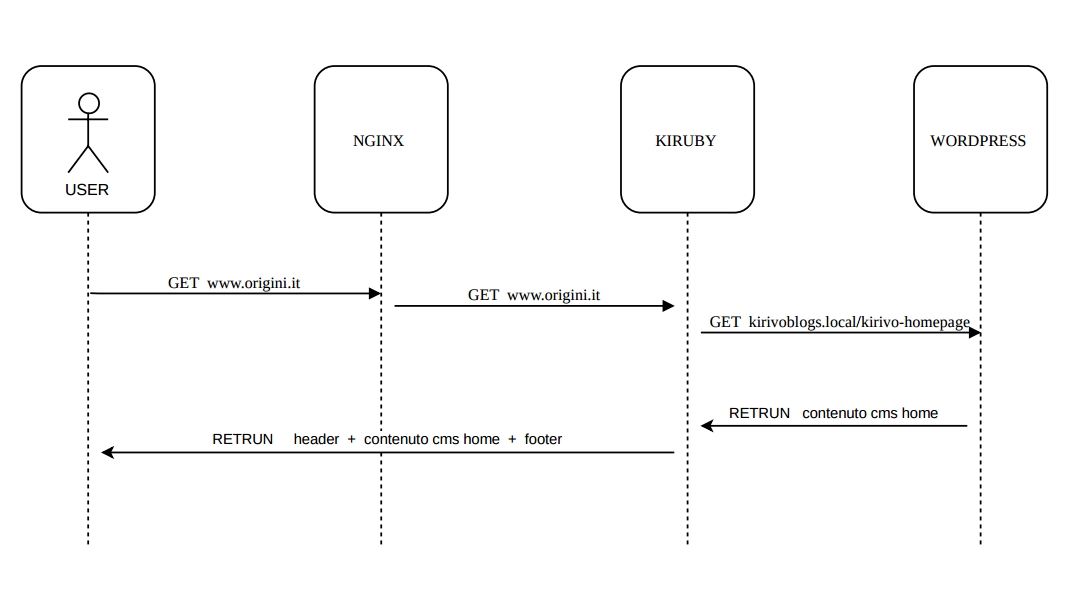
\includegraphics[width=\textwidth]{figure/homeseq.png}
  \caption{Funzionamento della richiesta della homepage.}
  \label{fig:homeseq}
\end{figure}



\section{La gemma cmsdealer}
Per visualizzare contenuti dinamici, come ad esempio un Box di 4 vini viene utilizzata
una gemma (così vengono chiamate in Ruby le librerie) chiamata \emph{cmsdealer}.

La gemma è necessaria per il fatto che le informazioni dei prodotti, come nome del venditore, prezzo, spese di spedizione ecc... non sono accessibili a Wordpress, che viene utilizzato
come server per la gestione e la modifica di contenuti editoriali, ma sono accessibili a Kiruby che ha al suo interno diversi
meccanismi per accedere alle informazioni dei prodotti andandosi ad interfacciare con Hybris e SolR.

La gemma \emph{cmsdealer} usata dal server Kiruby scansiona la pagina di Wordpress da includere,
se incontra un tag di nome \emph{dynamic} ne legge l'attributo \emph{type} e in base al valore di questo
seleziona il corrispondente template, legge l'ID dei prodotti e sostiusice al tag \emph{dyanmic} l'HTML del box con
i valori dei prodotti selezionati

Esempio: se processando la pagina HTML di Wordpress Kiruby trova
\begin{verbatim}
	<dynamic type="KirivoListingBox" ids="3422,2345,2872,2209" />
\end{verbatim}
allora verrà cercato il template di \emph{kirivolistingbox.html.erb} e verrà popolato
coi valori dei prodotti con gli identificativi specificati nell attributo \emph{ids}.


\begin{figure}
  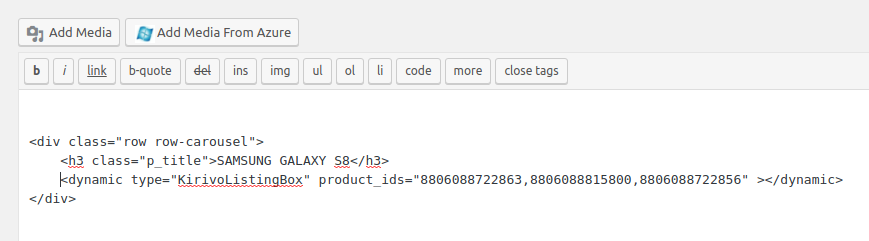
\includegraphics[width=\textwidth]{figure/sms-html.png}
  \caption{L'interfaccia visualizzata dai content managers per modificare un listing di prodotti.}
  \label{fig:smshtml}
\end{figure}

\begin{figure}
  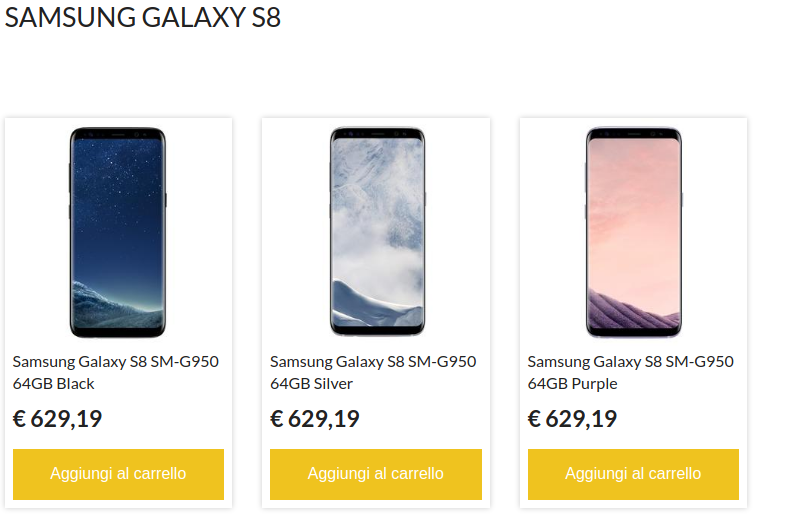
\includegraphics[width=\textwidth]{figure/sms-render.png}
  \caption{Risultato renderizzato della componente compilata in figura \ref{fig:smshtml}.}
  \label{fig:smsrender}
\end{figure}


\newpage

\section{Obbiettivo}
L'obbiettivo del progetto è quello di rendere l'edit delle pagine
da parte dei content molto più semplice e flessibile,
facendo in modo che i contenuti delle homepage possano essere editati visualmente e senza
modificare direttamente il codice HTML (vedi figure \ref{fig:meseform} e \ref{fig:smsform}).

Per farlo i content dovranno interagire con un interfaccia grafica web che permette
la modifica delle informazioni necessarie e di poter spostare e copiare
componenti della home con un click o con un drag and drop.


\begin{figure}
  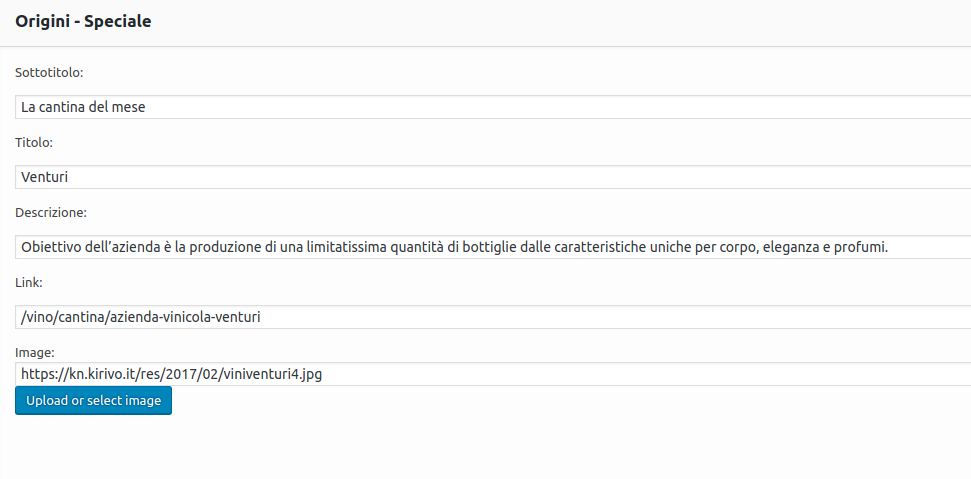
\includegraphics[width=\textwidth]{figure/wform.png}
  \caption{Come dovrebbe essere editata la componente in figura \ref{fig:wrender}.}
  \label{fig:meseform}
\end{figure}

\begin{figure}
  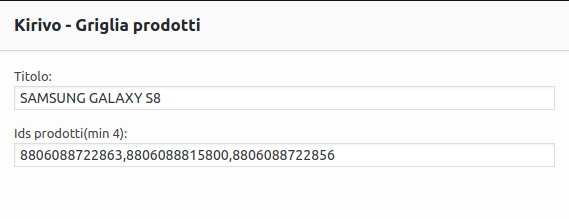
\includegraphics[width=\textwidth]{figure/sms-form.png}
  \caption{Come dovrebbe essere editata la componente in figura \ref{fig:smsrender}.}
  \label{fig:smsform}
\end{figure}

\section{Obbiettivo secondario}
Obbiettivo secondario del progetto e di rendere il sito più manutenibile.

La criticità del sistema è che contiene codice duplicato di componenti HTML nella gemma CmsDealer, in Kiruby
e nei widget di Wordpress. 

Per risolvere il problema sono state create le  \emph{RenderdPricesAPI} 
che restituiscono frammenti di HTML renderizzato per le varie componenti della home che contengono prodotti.

In questo modo il codice del template resta solamente in Kiruby e esponendo le 
API questo viene usato sia dai Widget di Wordpress sia dalla gemma CmsDealer.